% !Mode:: "TeX:UTF-8"
% !TEX root = tjumain.tex

\iffalse
\bibliography{reference/reference.bib} % 欺骗latextools获取bib文件
\fi

%%%%%%% 正文 %%%%%%%

\chapter{一个测试}

\section{真的只是一个测试}

中文学位论文测试\cite{chandrasekhar2003newton,arnold1990huygens}。

\subsection{参考文献标引}

一只敏捷的棕色狐狸跳过那只懒惰的狗\cite{chandrasekhar2003newton,arnold1990huygens}。

\chapter{继续测试}

\section{行内公式与行间公式}

考虑整个供应链的利润函数$\beta_{SC}$。因为$\frac{\partial\beta_{SC}}{\partial p_1}=q-\int_0^q F(x)\ud x>0$,所以$\beta_{SC}$对$p_1$单调递增,所以:
\begin{equation}
\label{dscNoStgProof0}
\beta_{SC}(q_s,p_{1s},p_{2s})<\beta_{SC}(q_s,p_{1n},p_{2n})
\end{equation}

因为对于$\forall q\in[q_s, q_n)$,有:
\[ \left.\frac{\partial \beta_{SC}}{\partial q}\right|_{(q,p_{1n},p_{2n})}=p_{1n}-c+c_L+(p_{2n}-p_{1n}-c_L)F(q) \]

销售商决策如式~\eqref{rcond}~所示:
\begin{equation}
\label{rcond}
\left\{\begin{array}{l}
p_{1s}=v_h-(v_h-p_2)\mathbb{E}(\varphi) \\
p_{2s}=v_l \\
q_s \in \underset{q \geq 0}{\mathrm{argmax}} \beta_R (q, p_1, p_2) \\
\end{array}\right.
\end{equation}

\section{插图}

当$q=5190$时,$p_{1s}=5.78,p_{2s}=2.95$,图像如图~\ref{fig:simuP1P2Result}~所示。
\begin{figure}[htbp!]
\centering
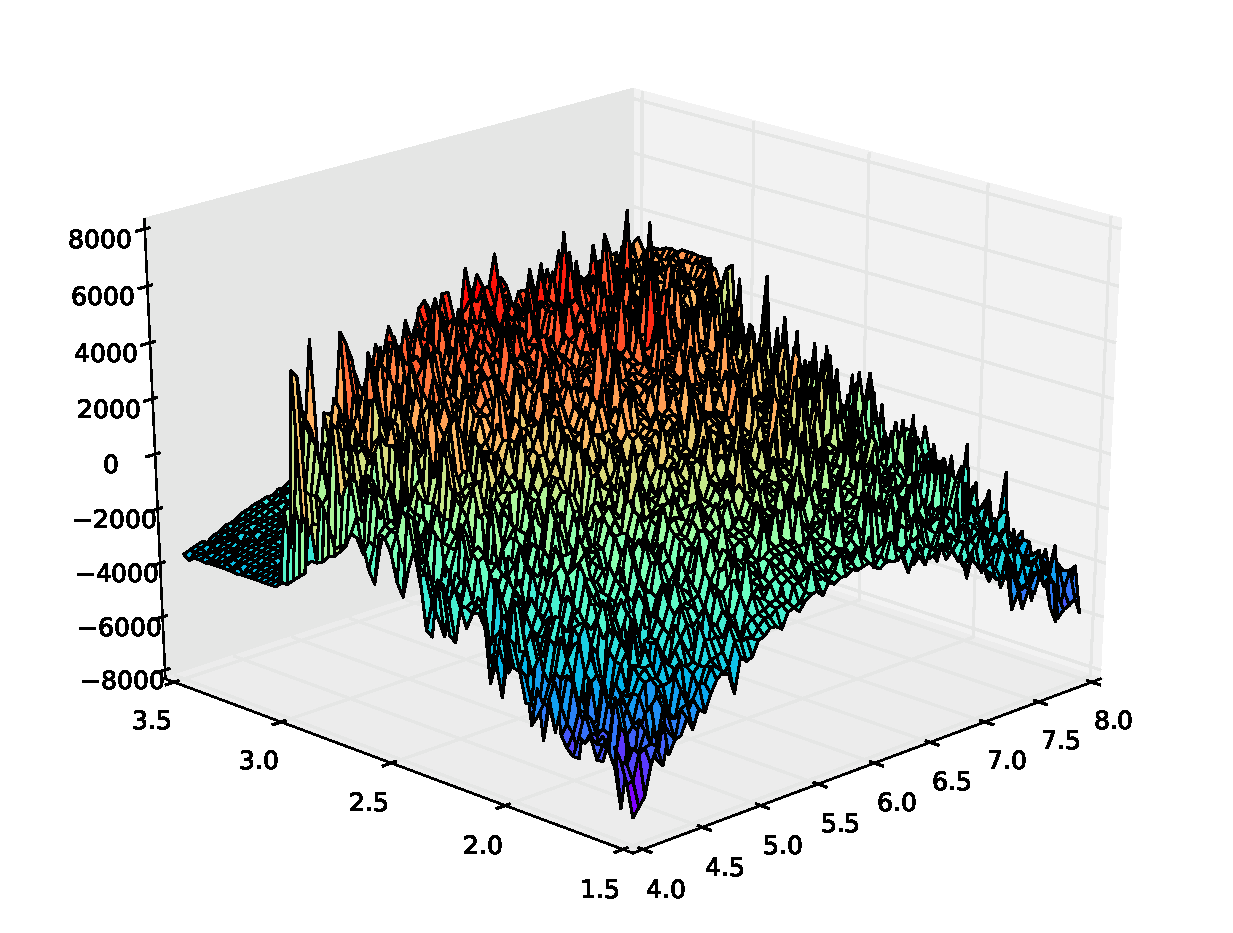
\includegraphics[width=0.75\textwidth]{figures/p1p2figure.eps}
\caption{最优$p_1, p_2$仿真结果}\label{fig:simuP1P2Result}
\vspace{-1em}
\end{figure}

\section{代码环境}

很多和计算机专业背景相关的同学都会使用到代码环境,使用~\verb|\verb|~指令或者是~\verb|verbatim|~环境固然是一种选择,但是比不上专门的~lstlisting~环境这么专业。

\begin{lstlisting}
int main(int argc, char ** argv) {
    printf("Hello world!\n");
    return 0;
}
\end{lstlisting}

\section{普通表格的绘制方法}

表格应具有三线表格式,其标准格式如表 \ref{tab:table1} 所示。
\begin{table}[htbp]
\caption{符合本科生毕业论文绘图规范的表格}\label{tab:table1}
\vspace{0.5em}\centering\wuhao
\begin{tabular}{ccccc}
\toprule[1.5pt]
$D$(in) & $P_u$(lbs) & $u_u$(in) & $\beta$ & $G_f$(psi.in)\\
\midrule[1pt]
 5 & 269.8 & 0.000674 & 1.79 & 0.04089\\
10 & 421.0 & 0.001035 & 3.59 & 0.04089\\
20 & 640.2 & 0.001565 & 7.18 & 0.04089\\
 5 & 269.8 & 0.000674 & 1.79 & 0.04089\\
10 & 421.0 & 0.001035 & 3.59 & 0.04089\\
20 & 640.2 & 0.001565 & 7.18 & 0.04089\\
 5 & 269.8 & 0.000674 & 1.79 & 0.04089\\
10 & 421.0 & 0.001035 & 3.59 & 0.04089\\
20 & 640.2 & 0.001565 & 7.18 & 0.04089\\
 5 & 269.8 & 0.000674 & 1.79 & 0.04089\\
10 & 421.0 & 0.001035 & 3.59 & 0.04089\\
20 & 640.2 & 0.001565 & 7.18 & 0.04089\\
\bottomrule[1.5pt]
\end{tabular}
\vspace{\baselineskip}
\end{table}